\section{Datapath}
This section describes the datapath and its internal elements. The datapath is the component that connects the pipeline components within itself as well as with cpu inputs and outputs and the controlpath.

This MIPS implementation works with a 5 stage pipeline in order to achieve a fast clock. The datapath consists of instruction fetch, instruction decode, execution, memory stage and writeback.
The datapath controls the information flow from one pipeline stage to the next with registers. 
These writing process occur on the positive edge of the clock when the pipeline stage input from the controlpath. That is, the registers forwards information synchronously. 
The datapath forwards the controlpath signals asynchronously, contrary to the pipeline to pipeline signals.



\begin{figure}
  \centering
  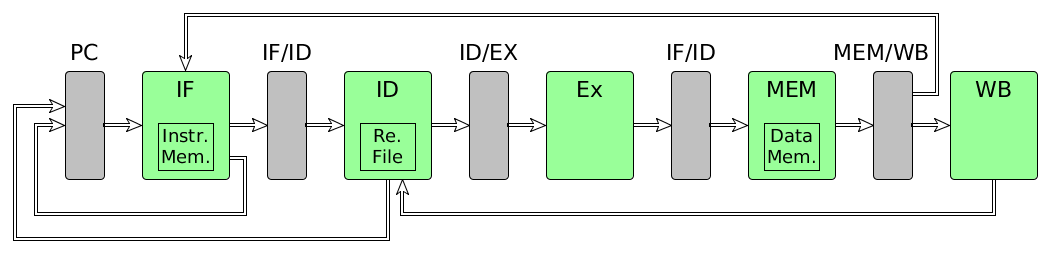
\includegraphics[width=0.8\textwidth]{figure/datapath.png}
  \caption{Datapath pipeline}
  \label{fig:datapath}
\end{figure}

The program counter (PC) is programmed into the datapath. Its function is the store the current program address, which is mostly counted up.
It has a multiplexer controlled by the controlpath to choose the input. The two possible inputs are to count up (PC+4) from instruction fetch
and the jump or branch from instruction decode. The controlpath chooses always the instruction decode input in the case of jump or branch. 
On the jump command, PC will receive the jump value. In case of a branch, PC will receive either the branch value or PC+4, 
depending on the instruction decode decision. This behaviour allows for the controlpath always to 
activate the instruction decode input in cases of jumps and branches.

The following subsections describe the pipeline components as well as its functions and IOs. 

\subsection{Instruction fecth}
This first block of the pipeline is the instruction fetch. The main task of this block is to fetch the next instruction and pass it further to the pipeline. 

The program counter is a 32-bit input, which is directly outputted as instruction address to fetch an instruction. The instruction fetch inputs the program memory's instruction data, 
with the actual 32-bit instruction. This value is directly forwarded to the pipeline.

The program counter is also incremented by four, because the used memory is 8-bit long. This incremented value is given back to PC.
\subsection{Instruction decode}
The second block of the pipeline if the instruction decode. Its main tasks are to divide the instruction into its pieces, manage the register file and manage branches.

\subsubsection{Register File}
The register file is a set of 32 general purpose 32-bit registers. These have the advantage, comparing to the ram memory, that they can always be accessed within one clock cycle.
The access to these registers is made with five bits, which allows multiple registers to be referenced per instruction. All loaded memory values are stored in a register
for later use.

The registers are numbered from \$0 through \$31. There is also a convention for using these registers, which must be enforced by assembly language and follow \autoref{tab:mips registers}:

\begin{table}[h!]
	\centering
	 \caption{MIPS registers}	
	\begin{tabular}{ccl}
		\toprule[2pt]
		\textbf{Register Number} & \textbf{Conventional Name} &\textbf{Usage}  \\
		\toprule[2pt]
		\$0 & \$zero & Hard-wired to 0 \\
		\$1 & \$at & Reserved for pseudo-instructions \\
		\$2 -\$3 & \$v0, \$v1 & Return values from functions \\
		\$4 - \$7 & \$a0 - \$a3 & Arguments fo functions - not preserved by subprograms \\
		\$8 - \$15 & \$t0 - \$t7 & Temporary data, not preserved by subprograms \\
		\$16 - \$23 & \$s0 - \$s7 & Saved registers, preserved by subprograms \\
		\$24 - \$25 & \$t8 - \$t9 & More temporary registers, nor preserved by subprograms  \\
		\$26 - \$27 & \$k0 - \$k1  & Reserved for kernel. Dot not use. \\
		\$28 & \$gp & Global Area Pointer (base of global data segment) \\
		\$29 & \$gp & Stack pointer \\
		\$30 & \$sp & Frame Pointer \\
		\$31 & \$ra & Return Address \\
		\bottomrule[2pt]
	\end{tabular} 
	\label{tab:iu_Kennlinie}
\end{table}

This implementation of MIPS does not have a FPU. In case of FPUs another 32 32-bit register set is used.
\subsubsection{Forwarding}
\subsubsection{Branch Logic}


\subsection{Execution}
\subsection{Memory Stage}
The memory stage is the fourth block of the pipeline and has the main task of fetch or save in the memory. 

For memory operations the execution stage outputs two 32-bit values: aluResult\_in, which works as the memory address, and data\_in, which is data to be written in the memory. 
On read operations, the data\_to\_cpu input delivers the 32-bit memory value.

This stage has one multiplexer choosing the pipeline stage output from aluResult\_in or data\_to\_cpu.
\subsection{Writeback}
This writeback stage is the fifth and last stage of the pipeline. Its main task is just to hold the calculated values, as well as the values read from the memory 
so they can be written the register file.
